\section{Physical quantities:unit\'a di misura e ordini di grandezza e scaling laws.}

\subsection{masses}

\begin{frame}{elementar masses}
    \begin{itemize}
\item $m_P=938.3\Mcs$
\item $m_N=939.7\Mcs$
\item $m_e=0.51\Mcs$
\item  $1 u=931.49 \Mcs$.
\end{itemize}
\end{frame}

\subsection{Interaction coupling}

\begin{frame}{costante struttura fine}
    $\alpha_{SF}=\frac{e^2}{(4\pi\epsilon_0)\hbar c}\approx\frac{1}{137}$.
\end{frame}

\subsection{Energie}

\begin{frame}{Energia in varie unit\'a}

Relazioni $u,c,MeV$:
 
$c^2=931.502\frac{MeV}{u}$.
 
$e^2=1.44\,MeV\,fm$.
 
Conversione eV-Kelvin:
 
\begin{align*}
1  ^{\degree}K&= 8.621738*10^{-5}  eV \\
&= 0.0862 meV \\
&= 0.695 cm^{-1}
\end{align*}

\begin{align*}
1 a.u=27.211396 eV=219474.63 cm^{-1}\\
1 Ry=13.6057 eV \\
1 eV =8065.54 cm^{-1} \\
1 eV= 11,600  ^{\degree}K\\
1 meV = 8.065 cm^{-1}
\end{align*}
\end{frame}

\subsection{lengths}

\begin{frame}{Borh radius, electron radius, Compton wavelength}
    The ratio of three characteristic lengths:

the classical electron radius $r_e=(\frac{1}{4\pi\epsilon_0})\frac{e^2}{m_ec^2}$, the Bohr radius $a_0=(4\pi\epsilon_0)\frac{\hbar^2}{m_ee^2}$  and the Compton wavelength of the electron $\lambdabar_e=\frac{\hbar}{m_ec}$:

$r_e=\frac{\alpha\lambda_e}{2\pi}=\alpha^2a_0$.
\end{frame}

\begin{frame}{Atom vs nucleus}
\begin{columns}[T]
\begin{column}{0.5\textwidth}
Atomo d'idrogeno:
    \begin{itemize}
        \item Raggio di Bohr.
$a_0=\frac{\hbar^2}{m_ee^2}=5.3*10^{-9} cm$
\item Magnetone di Bohr.
SI: $\mu_B=\frac{e\hbar}{2m_e}=5.788*10^{-5}eV*T^{-1}$.
cgs: $\mu_B=\frac{e\hbar}{2m_ec}$.
atomic unit: $\frac{\alpha}{2}$
\item  Livelli energetici $E_n=\frac{m_ec^2\alpha^2}{2n^2}=\frac{13.6eV}{n^2}$.
    \end{itemize}
\end{column}
\begin{column}{0.5\textwidth}
    \begin{itemize}
        \item    raggio nucleare
        \item Magnetone nucleare
SI $\mu_N=\frac{e\hbar}{2m_pc}=3.15245*10^{-8}eV*T^{-1}=\frac{\mu_B}{1836}$.
\item Momento di quadrupolo.
\item Deutone.
\begin{align*}
&B=2.22 MeV\\
&\mu_d=0.8574376\mu_N\\
&S=1\\
&Q=2.8*10^{-27}cm^2=0.28fm^2(Q_{zz})\\
&=\frac{2}{5}eZ(b^2-a^2)
\end{align*}
\item barn $=10^2 fm^2=10^{-24}cm^2$
    \end{itemize}
\end{column}
\end{columns}
\end{frame}

\section{Math memo}

\subsection{Identities}

\begin{frame}{Calcolo vettoriale}
    \begin{align*}
    &\nabla\wedge(\nabla\wedge\vec{A})=\nabla(\scap{\nabla}{A})-\nabla^2\vec{A}\\
    &\rot{\vecp{A}{B}}=(\scap{B}{\nabla})\vec{A}-(\scap{A}{\nabla})\vec{B}+\vec{A}\div{\vec{B}}-\vec{B}\div{\vec{A}}
    \end{align*}
\end{frame}

\begin{frame}{Usefull Derivatives}
    \begin{align*}
        &\nabla(\frac{1}{|\vec{x}-\vec{x}'|})=-\frac{\vec{x}-\vec{x}'}{|\vec{x}-\vec{x}'|^3}
    \end{align*}
\end{frame}

\begin{frame}{trigo}
T. del coseno (Carnot) $a^2=b^2+c^2-2ab\cos{\alpha}$.

$c=b\tan{\gamma}$.

$\tan{(\frac{\pi}{2}-\theta)}=\cot{\theta}$

\end{frame}

\begin{frame}{Integrali}
$\int\frac{-1f'}{\sqrt{a^2-f^2(x)}}dx=\arccos{\frac{f}{a}}$

\end{frame}

\subsection{Equazioni differenziali}

\begin{frame}{prim'ordine}
    \begin{itemize}
        \item Equazione differenziale $\frac{dn_2}{dt}+P(t)n_2=Q(t)$\\
$n_2=\exp{-\int Pdt}[\int\exp{\int Pdt}Qdt+C]$
    \end{itemize}
\end{frame}

\subsection{Identit\'a integro-differenziali}

\begin{frame}{Coordinate sferiche}

Parte angolare di $\nabla^2$ in coordinate sferiche:
\begin{align*}
&\nabla^2=\frac{1}{r^2}[\nabla_r^2+\nabla_{\theta,\phi}^2]\\
&\nabla_r^2=\frac{\partial}{\partial r}(r^2\frac{\partial}{\partial r})\\ 
&\nabla_{\theta,\phi}^2=\frac{1}{\sin{\theta}}\frac{\partial}{\partial \theta}(\sin{\theta}\frac{\partial}{\partial \theta})+\frac{1}{\sin^2{\theta}}\frac{\partial^2}{\partial\phi^2}=-\frac{l^2}{\hbar^2}
\end{align*}

Gradient in spherical coordinates:
\begin{align*}
&\nabla=\hat{e_{r}}\frac{\partial}{\partial r}+\hat{e_{\theta}}\frac{1}{r}\frac{\partial}{\partial \theta}+\hat{e_{\phi}}\frac{1}{r\sin{\theta}}\frac{\partial}{\partial \phi}\\
&\hat{n}\cdot\vec{\nabla}=\frac{\vec{x}\cdot\vec{\nabla}}{r}=\frac{\partial}{\partial r}
\end{align*}

\end{frame}

\begin{frame}{Identit\'a di Green e teoremi di Stokes}
Green's second identity:
\begin{align*}
&\int_V(f_1\nabla^2f_2-f_2\nabla^2f_1)d^3x=\oint_S(f_1\nabla f_2-f_2\nabla f_1)\hat{n}ds
\end{align*}
\end{frame}

\subsection{funzione di Green}



\subsection{Funzioni speciali}

\begin{frame}{Funzioni di Bessel sferiche}
$j_l(x)=(\frac{\pi}{2x})^{\frac{1}{2}}J_{l+\frac{1}{2}}(x)$\lbt{\abc{x\rightarrow+\infty}\frac{1}{x}\sin{[x-\frac{l\pi}{2}]}}{\abc{x\rightarrow0}\frac{x^l}{(2l+1)!!}}\\
$n_l(x)=(-1)^{l+1}(\frac{\pi}{2x})^{\frac{1}{2}}J_{-l-\frac{1}{2}}(x)$\lbt{\abc{x\rightarrow+\infty}-\frac{1}{x}\cos{[x-\frac{l\pi}{2}]}}{\abc{x\rightarrow0}-\frac{(2l-1)!!}{x^{l+1}}}\\
$J_{\nu}$, $J_{-\nu}$ sono le funzioni di Bessel di ordine $\nu$ soluzioni di \\
$\frac{d^2R}{dx^2}+\frac{1}{x}\frac{dR}{dx}+(1-\frac{\nu^2}{x^2})R=0$ (Equazione di Bessel);\\
 se $\nu$ non \'e intero le due soluzioni sono indipendenti.
\textbf{$l=0$}: $j_0(x)=\frac{\sin{x}}{x}$, $n_0(x)=-\frac{\cos{x}}{x}$
(leggi $x=kr$)

\end{frame}


\begin{frame}{Spherical Hankel functions}
\lbt{h_l^{(1)=j_l+in_l}}{h_l^{(2)=j_l-in_l}} a ragione del fatto che \lbt{h_l^{(1)}\abc{\text{r grande}}\frac{e^{i(kr-l\frac{\pi}{2})}}{ikr}}{h_l^{(2)}\abc{\text{r grande}}\frac{e^{-i(kr-l\frac{\pi}{2})}}{ikr}}\\
    
\end{frame}

\begin{frame}{Legendre/Armoniche sferiche}
Legendre
 $P_l(x)=\frac{1}{2^ll!}(\frac{d}{dx})^l(x^2-1)^l$\\
\textbf{Ortogonalit\'a}: $\int_{-1}^1P_m(\cos{\theta})P_n(\cos{\theta})d(\cos{\theta})=\frac{2}{2n+1}\delta_{mn}$\\

Armoniche sferiche
Cerco soluzioni di \\
$\nabla^2f=\frac{1}{r^2}\frac{\partial}{\partial r}(r^2\frac{\partial f}{\partial r})=0$.\\
Separazione variabili $f(r,\theta,\phi)=R(r)Y(\theta,\phi)$:\\
\lbt{\frac{1}{R}\frac{d}{dr}(r^2\frac{dR}{dr})=\lambda}{\frac{1}{Y}\frac{1}{\sin{\theta}}\frac{\partial}{\partial \theta}(\sin{\theta}\frac{\partial Y}{\partial \theta})+\frac{1}{Y}\frac{1}{\sin^2{\theta}}\frac{\partial^2Y}{\partial \phi^2}=-\lambda};\\
ancora assumo $Y(\theta,\phi)=\Theta(\theta)\Phi(\phi)$:\\
\lbt{\frac{1}{\Phi(\phi)}\frac{d^2\Phi(\phi)}{d\phi^2}=-m^2}{\lambda\sin^2{\theta}+\frac{\sin{\theta}}{\Theta(\theta)}\frac{d}{d\theta}[\sin{\theta}\frac{d\Theta}{d\theta}]=m^2}.\\
${Y_l}^m(\theta,\phi)=(-1)^m\sqrt{\frac{2l+1}{4\pi}\frac{(l-m)!}{(l+m)!}}{P_l}^m(\cos{\theta})e^{im\phi}$\\
normalizzate secondo $\int d\theta\int d\phi {Y_l}^m{Y_l'}^{m'*}=\delta_{ll'}\delta_{mm'}$.

Teorema di addizione\\
$\sum_mY_l^m(\hat{r}){Y_l^m(\hat{h})}^*=[\frac{(2l+1)}{4\pi}]P_l(\hat{r}\cdot\hat{k})$
    
\end{frame}

\section{Elettromagnetismo}

\begin{frame}{Equazioni di Maxwell}

\begin{columns}
\begin{column}{0.5\textwidth}
    \begin{block}{Gaussian (cgs)}
\begin{align*}
&\epsilon_0=\mu_0=1\\
&\vec{D}=\vec{E}+4\pi\vec{P}\quad\vec{H}=\vec{B}-4\pi\vec{M}\\
&\vec{B}=\vecp{\nabla}{A}\\
&\vec{E}=-\nabla\phi-\frac{1}{c}\PDy{t}{\vec{A}}
\end{align*}    
    \end{block}
\end{column}
\begin{column}{0.5\textwidth}
        \begin{block}{SI}
\begin{align*}
&\epsilon_0=\frac{\num{e7}}{4\pi c^2}[I^2t^4m\expy{-1}l\expy{-3}]\ \mu_0=\frac{1}{\epsilon_0c^2}\\
&\vec{D}=\epsilon_0\vec{E}+\vec{P}\quad\vec{H}=\frac{1}{\mu_0}\vec{B}-\vec{M}\\
&\vec{B}=\vecp{\nabla}{A}\\
&\vec{E}=-\nabla\phi-\PDy{t}{\vec{A}}
\end{align*}    
    \end{block}
\end{column}
\end{columns}
\begin{columns}
\begin{column}{0.5\textwidth}
    \begin{block}{Equazioni di Maxwell (cgs)}
\begin{align*}
    &\div{\vec{B}}=0\\
    &\div{\vec{E}}=4\pi\rho_c\\
    &\rot{\vec{E}}=-\frac{1}{c}\PDy{t}{\vec{B}}\\
    &\rot{\vec{B}}=\frac{1}{c}\PDy{t}{\vec{E}}+\frac{4\pi}{c}\vec{j}_c
\end{align*}    
    \end{block}
\end{column}
\begin{column}{0.5\textwidth}
        \begin{block}{Equazioni di Maxwell (SI)}
\begin{align*}
    &\div{\vec{B}}=0\\
    &\div{\vec{D}}=\rho_c\\
    &\rot{\vec{E}}=-\PDy{t}{\vec{B}}\\
    &\rot{\vec{H}}=\PDy{t}{\vec{E}}+\vec{j}_c
\end{align*}    
    \end{block}
\end{column}
\end{columns}

\end{frame}

\begin{frame}{Sistema di cariche in campo esterno: Espansione in multipoli}
\begin{block}{Energia sistema di cariche localizzato in campo esterno}
\begin{align*}
    &\phi=\phi^{(0)}+\phi^{(1)}+\phi^{(2)}+\ldots \quad \phi^{(l)}=\frac{1}{r^{l+1}}\sum_{-l}^l\sqrt{\frac{4\pi}{2l+1}}Q_m^{(l)}Y_{lm}^*(\theta,\phi)\\
    &Q_m^{(l)}=\sqrt{\frac{4\pi}{2l+1}}\int Y_{lm}(\theta',\phi')r'^l\rho(\vec{x}')\,d^3x',\ Q_0^{(1)}=id_z,\ Q_0^{(2)}=-\frac{1}{2}D_{zz},\ldots\\
    &W=\int\rho(\vec{x})\phi(\vec{x})d^3x=q\phi(0)-\scap{p}{E}(0)-\frac{1}{6}\sum_{ij}Q_{ij}\PDy{x_i}{E_j}(0)+\ldots
\end{align*}
\end{block}
\begin{block}{Localized current distribution in external magnetic induction}
\begin{align*}
    &F_i=\sum_{jk}\epsilon_{ijk}[B_k(0)\int J_j(\vec{x}')\,d^3x'+\int J_j(\vec{x}')\vec{x}'\cdot\nabla B_k(0)\,d^3x'+\ldots]\\
    &\vec{F}=\nabla(\scap{m}{B})(NEM: +\frac{1}{c^2}\TDof{t}(\vecp{E}{m}))\quad cB/L(E/\lambdabar)\\
    &\vec{N}=\vecp{m}{B}(0)\ U=-\scap{m}{B}
\end{align*}
\end{block}
\end{frame}

\begin{wordonframe}{cose su potenziali em}

Equazione di Poisson per il potenziale elettrico $\nabla^2 V(r)=-4\pi \rho (-\frac{\rho}{\epsilon_0})$

\end{wordonframe}

\begin{frame}{Sistema di cariche in campo esterno: potenziale vettore}

        \begin{block}{Potenziale vettore: campo magnetico costante}
    \begin{align*}
        &\vec{B}(\vec{x})=\vecp{\nabla}{A}(\vec{x})\\
        &\nabla^2\vec{A}=-\frac{4\pi}{c}\vec{j}(\text{Coulomb gauge})\\ &\vec{A}=\frac{1}{c}\int\,d^3x'\frac{\vec{j}}{|\vec{x}-\vec{x}'|}
    \end{align*}
    \end{block}
   
       \begin{columns}[T]
       \begin{column}{0.5\textwidth}
        \begin{block}{Campo magnetico medio a grande distanza}
        Sviluppo in serie di potenze di $\vec{x}'$:
        \begin{align*}
            &\vec{m}=\frac{1}{2(c)}\sum e\vecp{x'}{v}\\
            &\vec{A}=\nabla(\frac{1}{r})\wedge\vec{m}\\
            &B(\vec{x})=(\frac{4\pi}{\mu_0})[\frac{3\hat{x}(\hat{x}\cdot\vec{m})-\vec{m}}{x^3}]
        \end{align*}
        \end{block}
   
       \end{column}
       \begin{column}{0.5\textwidth}
            \begin{block}{Magnetic dipole (Classical picture)}
\begin{align*}
    &|\vec{\mu}|=\frac{e}{(\frac{2\pi r}{v})}\pi r^2=\frac{evr}{2}=\frac{e}{2m(c)}|\vec{l}|\\
    &\vec{\mu}=\frac{1}{2}\int\vecp{r}{\vecp{\nabla}{M}}d^3x\\
    &=\frac{1}{2c}\int(\vecp{r}{j})d^3x'
\end{align*}
\end{block}
       \end{column}
       \end{columns}

    
\end{frame}

\begin{frame}{Electric and magnetic dynamics}
\begin{block}{Systems of charges and currents in free space}
\begin{align*}
&W=\frac{1}{2}\int\phi\rho\,d^3x\to\delta W=\int\vec{E}\cdot\delta\vec{D}\,d^3x\\
&W=\frac{1}{2}\int\scap{J}{A}\,d^3x\to\frac{1}{2}\int_{V_1}\vec{M}\cdot\vec{B}_0\,d^3x
\end{align*}
\end{block}
\begin{block}{Forza di Lorenz (per unit\'a di carica)}
\begin{columns}[T]
\begin{column}{0.5\textwidth}
$\vec{E}+\frac{\vec{v}}{c}\wedge\vec{B}$
\end{column}
\begin{column}{0.5\textwidth}
$\vec{E}+\vec{v}\wedge\vec{B}$
\end{column}
\end{columns}
\end{block}
\begin{block}{Teorema di Larmor}
Il comportamento di un sistema di cariche in moto finito avente lo stesso $e/m$ in campo elettrico a simmetria centrale e campo magnetico debole e uniforme \'e equivalente allo stesso sistema senza campo magnetico in riferimento ratante $\vec{\Omega}=\frac{e\vec{H}}{2mc}$ (frequenza di Larmor).


\end{block}
\end{frame}

\begin{frame}{Gauge freedom}

 \begin{block}{Gauge di Coulomb: $\div{\vec{A}}=0$}
\begin{columns}[T]
\begin{column}{0.5\textwidth}
        \begin{align*}
            &\frac{1}{c^2}\nabla\PDy{t}{\phi}=(\mu_0)\vec{J}_l\\
            &\nabla^2\vec{A}-\frac{1}{c^2}\PtwoDy{t}{\vec{A}}=-(\mu_0)\vec{J}_t
        \end{align*}
   
\end{column}
\begin{column}{0.5\textwidth}
Instantaneous Coulomb potential
\begin{equation*}
\phi(\vec{x},t)=(\frac{1}{4\pi\epsilon_0})\int\frac{\rho(\vec{x}',t)}{|\vec{x}-\vec{x}'|}\,d^3x'
\end{equation*}
Transverse current:
\begin{align*}
    &\vec{J}_t=\frac{1}{4\pi}\nabla\wedge\nabla\wedge\int\frac{\vec{J}}{|\vec{x}-\vec{x}'|}\,d^3x'\\
    &\nabla^2\vec{A}-\frac{1}{c^2}\PDy{t}{\vec{A}}=-(\mu_0)\vec{J}_t
\end{align*}
\end{column}
\end{columns}
        \end{block}
  \begin{block}{Lorenz condition (vacuum)}
\begin{columns}[T]
\begin{column}{0.5\textwidth}
    \begin{align*}
        &\nabla\cdot\vec{A}+\frac{1}{c^2}\PDy{t}{\phi}=0\\
        &\PDy{x_k}{A_k}=0
    \end{align*}
\end{column}
\begin{column}{0.5\textwidth}
\begin{align*}
    &()
\end{align*}
\end{column}
\end{columns}
    \end{block}

\end{frame}

\subsection{Radiazione EM}

\begin{frame}{Onde piane}
    
\end{frame}

\begin{frame}{Green function for wave equation}
    \begin{block}{Helmholtz wave equation}
    \begin{columns}[T]
    \begin{column}{0.5\textwidth}
    \begin{align*}
    &\nabla^2\psi-\frac{1}{c^2}\PtwoDy{t}{\psi}=-4\pi f(\vec{x},t)\\
    &(\nabla-\frac{1}{c^2}\PtwoDof{t})G^{(\pm)}(\vec{x},t;\vec{x}',t')=\\
    &4\pi\delta(\vec{x}-\vec{x}')\delta(t-t')\\
    &G^{(\pm)}(\vec{x},t;\vec{x}',t')=\frac{\delta(t'-[t\mp\frac{|\vec{x}-\vec{x}'|}{c}])}{|\vec{x}-\vec{x}'|}\\
    &\psi(\vec{x},t)=\psi_{in}(\vec{x},t)\\
    &+\iint G^{(\pm)}(\vec{x},t;\vec{x}',t')f(\vec{x}',t')\,d^3x'\,dt'
    \end{align*}    
    \end{column}
    \begin{column}{0.5\textwidth}
    \begin{align*}
    &(\nabla^2+k^2)\psi(\vec{x},\omega)=-4\pi f(\vec{x},\omega)\\
    &(\nabla^2+k^2)G_k(\vec{x},\vec{x}')=-4\pi\delta(\vec{x}-\vec{x}')\\
    &G_k^{(\pm)}(|\vec{x}-\vec{x}'|=R)=\frac{\exp{\pm ikR}}{R}
    \end{align*}    
    \end{column}

    \end{columns}
    \end{block}
\end{frame}

\section{Relativit\'a: formalismo covariante.}

\subsection{Invarianza della velocit\'a della luce}

\begin{frame}{Trasformazioni di Lorentz}
    \begin{columns}[T]
    \begin{column}{0.4\textwidth}
\begin{block}{Equazione d'onda}
\begin{equation*}
   (\nabla^2-\frac{1}{c^2}\PDof{t})\psi=0 
\end{equation*}
Non \'e invariante in forma per trasformazioni di Galilei.
\end{block}
    \end{column}
    \begin{column}{0.6\textwidth}
    \begin{block}{L'intervallo tra due eventi \'e uguale in tutti i riferimenti inerziali}
    \begin{equation*}
        ds^2=c^2\,dt^2-dx^2-dy^2-dz^2=ds'^2
    \end{equation*}
    \end{block}
    \end{column}
    \end{columns}
    \begin{align*}
        &x=x'\cosh{\psi}+ct'\sinh{\psi},\ ct=x'\sinh{\psi}+ct'\cosh{\psi},\ \tanh{\psi}=\frac{V}{c}\\
        &x=\frac{x'+Vt'}{\sqrt{1-\frac{V^2}{c^2}}}=\gamma(x'+\beta ct'),\ ct=\frac{ct'+\frac{V}{c}x'}{\sqrt{1-\frac{V^2}{c^2}}}=\gamma(ct'+\beta x')
    \end{align*}
\end{frame}

\begin{frame}{Elettrodinamica covariante}
    
\end{frame}



\section{QM}
%$\Delta p*\Delta x\geq\frac{\hbar}{2}$
%% http://www.dfa.unict.it/home/lombardo/images/cap_15.pdf teorema proiezione

\begin{frame}{Equazione d'onda di Schr\"oedinger}

\begin{columns}[T]
\begin{column}{0.5\textwidth}
\begin{block}{ES}
\begin{align*}
    &i\hbar\PDy{t}{\psi}=-\frac{\hbar^2}{2m}\nabla^2\psi+U\psi\\
    &E_n:\quad \frac{\hbar^2}{2m}\nabla^2\psi+[E-U]\psi=0
\end{align*}
\end{block}

\end{column}
\begin{column}{0.5\textwidth}
\begin{block}{Limite classico ($\hbar\to0$)}
\begin{align*}
    &\psi=a\exp{\frac{iS}{\hbar}} \leftrightarrow |\psi|^2=a^2,\frac{\nabla S}{m}=\frac{\vec{p}}{m}\\
    &\PDy{t}{a^2}+\div{(a^2\frac{\nabla S}{m})}=0
\end{align*}
\end{block}
\end{column}

\end{columns}

\begin{block}{Leggi di trasformazione di $\psi$ per trasformazione di Galilei}
Onde piane nei sistemi K e K' con K' in moto rispetto a K con velocit\'a $\vec{V}$:
\begin{align*}
    &\psi(\vec{r},t)\propto\exp{i(\scap{p}{r}-Et)/\hbar}\quad \psi'(\vec{r}',t)\propto\exp{i(\vec{p}'\cdot\vec{r}'-E't)/\hbar}\\
    &\vec{p}=\vec{p}'+m\vec{V}\quad E=E'+\vec{V}\cdot\vec{p}'+\frac{mV^2}{2}\\
    &\psi(\vec{r},t)=\psi'(\vec{r}',t)\Exp{i/\hbar(m\vec{V}\cdot\vec{r}'+\frac{mV^2}{2}t)}\\
    &=\psi'(\vec{r}-\vec{V}t,t)\Exp{i/\hbar(m\vec{V}\cdot\vec{r}-\frac{mV^2}{2}t)}
\end{align*}
\end{block}

\end{frame}

\begin{frame}{Problemi unidimensionali}
    
\end{frame}

\begin{frame}{Campo centrale}
    \begin{block}{ES in coordinate sferiche}
Operatore momento angolare $L^2$ in coordinate polari:

$L^2=-\hbar^2[\frac{1}{\sin{\theta}}\frac{\partial}{\partial \theta}(\sin{\theta}\frac{\partial}{\partial \theta})+\frac{1}{\sin^2{\theta}}\frac{\partial^2}{\partial \phi^2}]$\\
La componente radiale della quantit\'a di moto:
\begin{align*}
&p_r\psi=-i\hbar\frac{1}{r}\frac{\partial}{\partial r}(r\psi)=-i\hbar(\frac{\partial}{\partial r}+\frac{1}{r})\psi\\
&-\frac{\hbar^2}{2m}\nabla^2=-\frac{\hbar^2}{2mr^2}\frac{\partial}{\partial r}(r^2\frac{\partial}{\partial r})+\frac{1}{2mr^2}L^2=\frac{p_r{p_r}^{}}{2m}+\frac{L^2}{2mr^2}
\end{align*}
\end{block}
\end{frame}

\begin{frame}{Corrente di probabilit\'a}

\textbf{Derivazione}\\
$\int_V(\psi^*\frac{\partial \psi}{\partial t}+\psi\frac{\partial \psi^*}{\partial t})d^3x=-\frac{i}{\hbar}\int_V(\psi^*H \psi+\psi H\psi^*)d^3x=-\frac{i\hbar}{2m}\int_V(\psi^*\nabla^2\psi+\psi\nabla^2\psi^*)d^3x$
\textbf{Expressions}\\
$\vec{J}=\frac{1}{2m}(\psi\vec{P}^*\psi^*+\psi^*\vec{P}\psi)=$\lbt{\frac{\hbar}{m}\Im{\psi^*\nabla\psi}}{\frac{1}{m}\Re{[\psi^*P\psi]}}\\
Scritto $\psi(\vec{x},t)=|\psi|e^{i\frac{S(\vec{x},t)}{\hbar}}$ ho $\vec{j}=\frac{1}{m}|\psi|^2\nabla S$\\
\textbf{Equazione di continuit\'a}\\
$\frac{d}{dt}\int |\psi|^2dV=-\int \nabla\cdot{\vec{J}} dV=-\oint_\Sigma \vec{J}\cdot d\vec{\sigma}$\\
\textbf{Corrente di probabilit\'a radiale } (Per abituarci introduciamo sc):\\
${j_r}^{sc}=\hat{n}\cdot\vec{j}^{sc}(\vec{x},t)=\frac{\hbar}{m}\Im [{\psi^{sc}}^*(\vec{x},t)\vec{n}\cdot\nabla\psi^{sc}(\vec{x},t)]=\frac{\hbar}{m}\Im [{\psi^{sc}}^*(\vec{x},t)\frac{\partial}{\partial r}\psi^{sc}(\vec{x},t)]$
\end{frame}

\begin{frame}{Autostati energia e momento angolare}

Stato d'onda sferica: autostato simultaneo di $H_0$, $\vec{L}^2$, $L_z$:\\
$\ket{Elm}$

Onde sferiche: rappresentazione nello spazio delle coordinate e degli impulsi\\
\lbt{\braket{\vec{k}|Elm}=\frac{\hbar}{\sqrt{mk}}\delta{(E-\frac{\hbar k^2}{2m})}Y_l^m(\hat{k})}{\braket{\vec{x}|Elm}=\frac{i^l}{\hbar}\sqrt{\frac{2mk}{\pi}}j_l(kr)Y_l^m(\hat{r})}\\

Raccordo fra base di onde piane $\ket{\vec{k}}$, e base onde sferiche $\ket{Elm}$:\\
$\braket{\vec{x}|\vec{k}}=\frac{\pw{k}{r}}{(2\pi)^{\frac{3}{2}}}=\sum_l\sum_m\int dE\braket{\vec{x}|Elm}\braket{Elm|\vec{k}}=\frac{1}{(2\pi)^{\frac{3}{2}}}\sum_l(2l+1)i^lJ_l(kr)P_l(\hat{k}\cdot\hat{r})$\\
$\braket{\vec{k}|Elm}=\frac{\hbar}{\sqrt{mk}}\delta(\frac{\hbar^2k^2}{2m}-E)Y_l^m(\hat{k})$.

Espansione di $\pw{k}{r}$ in armoniche sferiche:
\begin{align*}
&\pw{k}{r}=e^{ikr\cos{\theta}}=\sum_{l=0}^{\infty}i^l(2l+1)J_l(kr)P_l(\cos{\theta})\\
&\pw{k}{r}=4\pi\sum_{l=0}^{\infty}i^lj_l(kr)\sum_{m=-l}^l{{Y_l}^m}^*(\theta_{\vec{k}},\phi_{\vec{k}}){Y_l}^m(\theta_{\vec{x}},\phi_{\vec{x}})
\end{align*}


\end{frame}

\begin{frame}{Commutatori J}
     Relazioni di commutazione per il momento angolare\\
$\vec{J}$ \index{Inserire: Definizione di J}\\
$[J_i,J_j]=i\hbar\bt{ijk}J_k$

 Relazioni per di commutazione per il momento angolare di spin (matrici di Pauli)\\
$\vec{S}=\frac{\hbar}{2}\vec{\sigma}$\\
$[S_i,S_j]=i\hbar\bt{ijk}S_k$\\
$\sigma_i^2=1$, $[\sigma_i,\sigma_j]=2i\bt{ijk}\sigma_k$, $\{\sigma_i,\sigma_j\}=2\delta_{ij}$\\
$(\scap{\sigma}{a})(\scap{\sigma}{b})=\scap{a}{b}+i\sigma\cdot(\vecp{a}{b})$
\end{frame}

\begin{frame}{ Operatori di rotazione e generatori.}
     
Esiste l'operatore di rotazione: $U_{\epsilon}=1-iG\epsilon$ con $G=\frac{J_k}{\hbar}$ e $\epsilon=d\phi$.

\begin{columns}[T]
\begin{column}{0.4\textwidth}
\begin{block}{Rotazioni infinitesime.}
\begin{align*}
&D(\hat{n},d\phi)=1-(\frac{\vec{J}\cdot\hat{n}}{\hbar})d\phi\\
&R_z(\epsilon)=\begin{pmatrix}1-\frac{\epsilon^2}{2}&-\epsilon&0\\\epsilon&1-\frac{\epsilon^2}{2}&0\\0&0&1\\\end{pmatrix}\\
&R_x(\epsilon)=\begin{pmatrix}0&0&1\\0&1-\frac{\epsilon^2}{2}&-\epsilon\\0&\epsilon&1-\frac{\epsilon^2}{2}\\\end{pmatrix}\\
&R_y(\epsilon)=\begin{pmatrix}1-\frac{\epsilon^2}{2}&0&\epsilon\\0&1&0\\-\epsilon&0&1-\frac{\epsilon^2}{2}\\\end{pmatrix}
\end{align*}
\end{block}
\end{column}
\begin{column}{0.6\textwidth}
\begin{block}{Operatori rotazione per spin $\frac{1}{2}$.}
\begin{align*}
&S_x=(\frac{\hbar}{2})[\ket{+}\bra{-}+\ket{-}\bra{+}]=(\frac{\hbar}{2})\sigma_x\\
&S_y=(\frac{i \hbar}{2})[-\ket{+}\bra{-}+\ket{-}\bra{+}]=(\frac{\hbar}{2})\sigma_y\\
&S_z=(\frac{\hbar}{2})[\ket{+}\bra{+}-\ket{-}\bra{-}]=(\frac{\hbar}{2})\sigma_z\\
&\sigma_x=\sigmax, \sigma_y=\sigmay,\\
&\sigma_z=\sigmaz\\
&D(\hat{n},\phi)=\exp{\frac{-i\vec{S}\cdot\hat{n}\phi}{\hbar}}=\exp{\frac{-i\vec{\sigma}\cdot\hat{n}\phi}{2}}\\
&\exp{\frac{-i\vec{\sigma}\cdot\hat{n}\phi}{2}}=\Id{2}\cos{(\frac{\phi}{2})}-i\vec{\sigma}\cdot\hat{n}\sin{(\frac{\phi}{2})}
\end{align*}
\end{block}
\end{column}
\end{columns}
\end{frame}

\begin{frame}{Atomo idrogenoide}
    
Tempo tipico: $\tau\approx \frac{2\pi\hbar^3}{m_ee^4}\approx1.5*10^{-16} s$.
 
Livelli energetici:
\begin{align*}
&\braket{n|H|n}=-\frac{E_{\text{Ryd}}}{n^2}Z^2\\ &E_{Ryd}=\frac{1}{(4\pi\epsilon_0)^2}\frac{me^4}{2\hbar^2}=\frac{1}{2}\alpha^2mc^2\approx13.6eV\\
&m=\frac{m_eM_P}{m_e+M_P}
\end{align*}

Dimensioni:
\begin{align*}
&r_B=(4\pi\epsilon_0 \text{ :SI})\frac{\hbar^2}{me^2}\approx0.529\angstrom (=5.29 \cdot10^{4} fm)\\ &\exv{r}=(\frac{r_B}{2Z}[3n^2-l(l+1)])\\ &\exv{r^2}=(\frac{r_B^2n^2}{2Z^2})[5n^2+1-3l(l+1)]\\ &\exv{\frac{1}{r}}=\frac{Z}{nr_b}
\end{align*}

\end{frame}

\begin{frame}{Autofunzioni dell'atomo idrogenoide}


\begin{itemize}
\item Livello $n=1$.

\begin{columns}
\begin{column}{0.5\textwidth}


Funzioni radiali:

$R_{1,0}=2\rho^\frac{3}{2}e^{-\rho}$.
\end{column}
\begin{column}{0.5\textwidth}

Armoniche sferiche:
$Y_{00}=\frac{1}{\sqrt{4\pi}}$.
\end{column}
\end{columns}

\item $n=2$.
\begin{columns}[T]
\begin{column}{0.5\textwidth}
Funzioni radiali:

\begin{align*}
&R_{2,0}=\frac{1}{\sqrt{2r_b^3}}(1-\frac{\rho}{2})e^{\frac{\rho}{2}}\\
&R_{2,1}=\frac{1}{\sqrt{24r_b^3}}\rho e^{\frac{\rho}{2}}
\end{align*}
\end{column}
\begin{column}{0.5\textwidth}
Armoniche sferiche:
\begin{align*}
&Y_{00}, Y_{10}=\frac{1}{2}\sqrt{\frac{3}{\pi}}\cos{\theta}\\
&Y_{1\pm1}=\mp\frac{1}{2}\sqrt{\frac{3}{2\pi}}\sin{\theta}e^{\pm i\phi}
\end{align*}
\end{column}
\end{columns}

\item $n=3$.
\begin{columns}
\begin{column}{0.5\textwidth}
Funzioni radiali:
\begin{align*}
&R_{30}=\frac{2}{\sqrt{27r_b^3}}[1-\frac{2}{3}\rho+\frac{2}{27}\rho^2]e^{-\frac{\rho}{3}}\\
&R_{31}=\frac{8}{27\sqrt{6r_b^3}}\rho [1-\frac{1}{6}\rho]e^{-\frac{\rho}{3}}\\
&R_{32}=\frac{4}{81\sqrt{30r_b^3}}\rho^2e^{-\frac{\rho}{3}}
\end{align*}
\end{column}
\begin{column}{0.5\textwidth}
Armoniche sferiche:
\begin{align*}
&Y_{00},Y_{10}, Y_{1\pm1}\\
&Y_{20}=\frac{1}{4}\sqrt{\frac{5}{\pi}}(2\cos^2{\theta}-\sin^2{\theta})\\
&Y_{2\pm1}=\mp\frac{1}{2}\sqrt{\frac{15}{2\pi}}\cos{\theta}\sin{\theta}\exp{\pm i\phi }\\
&Y_{2\pm2}=\frac{1}{4}\sqrt{\frac{15}{2\pi}}\sin^2{\theta}\exp{\pm2i\phi}
\end{align*}
\end{column}
\end{columns}
\end{itemize}

\end{frame}

\begin{frame}{Angoli eulero}
$\ket{\hat{n}}=D(R)\ket{\hat{z}}$ e $D(R)$ rappresenta una rotazione prima attorno a $y$ di $\theta$ e seguita da una attorno a $z$ di $\phi$ quindi $D(R)=D(\alpha=\phi,\beta=\theta,\gamma=0)$:\\
$D(\alpha, \beta, \gamma)=D_z(\alpha)D_y(\beta)D_z(\gamma)=\exp{\frac{-\sigma_3\alpha}{2}}\exp{\frac{-i\sigma_2\beta}{2}}\exp{\frac{-i\sigma_3\gamma}{2}}$
\end{frame}

\begin{frame}{Composizione momenti angolari. Coefficienti di CG}

In generale $[J_{1i}, J_{1j}]=i\hbar\bt{ijk} J_{1k}$, $[J_{2i}, J_{2j}]=i\hbar \bt{ijk} J_{2k}$ (useremo soprattutto  $[L_i,L_j]=i\hbar \bt{ijk} L_k$, $[S_i,S_j]=i\hbar\bt{ijk} S_k$: possiamo scegliere una base di
\begin{itemize}
\item Autoket simultanei di $\vec{J_1}^2$, $\vec{J_2}^2$, $J_{1z}$, $J_{2z}$.
 denotati con $\ket{J_1,J_2,J_{1z},J_{2z}}=\ket{J_1,J_2,m_1,m_2}$ 
\item Autoket simultanei di $\vec{J_1}^2$, $\vec{J_2}^2$, $\vec{J}^2$, $J_z$
 denotati con $\ket{J_1,J_2,J,J_z}$ 
\end{itemize}
Uso l'identit\'a $\sum_{m_1,m_2}\ket{J_1,J_2,m_1,m_2}\bra{J_1,J_2,m_1,m_2}=1$:

$\ket{J_1,J_2;J,M}\sum_{m_1,m_2}\ket{J_1,J_2;m_1,m_2}\underbrace{\braket{J_1,J_2;m_1,m_2|j_1j_2;JM}}_{CCG}$.

Stato d'onda sferica: autostato simultaneo di $H_0$, $\vec{L}^2$, $L_z$.\\
$\ket{Elm}$: Onde sferiche: rappresentazione nello spazio delle coordinate e degli impulsi\\
\lbt{\braket{\vec{k}|Elm}=\frac{\hbar}{\sqrt{mk}}\delta{(E-\frac{\hbar k^2}{2m})}Y_l^m(\hat{k})}{\braket{\vec{x}|Elm}=\frac{i^l}{\hbar}\sqrt{\frac{2mk}{\pi}}j_l(kr)Y_l^m(\hat{r})}.

Parit\'a: $(r,\theta,\phi)\abc{\pi}(r,\pi-\theta,\phi+\pi)$, $\spha{l}{m}(\pi-\theta,\phi+\pi)\rightarrow(-)^l\spha{l}{m}(\theta,\phi)$.

\end{frame}

\begin{frame}{Operatori tensoriali}

\begin{block}{Operatori di multipolo}
    Electric moments: Quadrupole\\
$Q(\psi)=\sum_{i=1}^Z\int e(3z_i^2-r_i^2)|\psi(\vec{x_1},\ldots,\vec{x_A})|^2d^3x$\\
In general $Q_{lm}=\int r^l{Y_{lm}}^*(\theta,\phi)\rho(x,y,z)d^3x$\\
\textbf{Momenti EM come componenti di un tensore sferico}\\
$Q_{lm}(\psi)=\sum_{i=1}^Z\int r^l{Y_{lm}}^*(\theta,\phi)|\psi(\vec{x_1},\ldots,\vec{x_A})|^2d^3x$:\\ $q=\sqrt{4\pi}Q_{0,0}$,\\ 
$D_Z=\sqrt{\frac{4\pi}{3}}Q_{1,0}$,\\
$Q=\sqrt{\frac{16\pi}{5}}Q_{2,0}$.
\end{block}

\begin{block}{Teorema di Wigner-Eckart}
$\braket{\alpha',j',m'|{T_q}^{(k)}|\alpha,j,m}=\braket{\alpha',j'||T^{(k)}||\alpha,j}*\braket{j,k;m,q|j,k;j',m'}$
    
\end{block}

Ho definito l'operatore di transizione come $V\ket{\psi^{(+)}}=T\ket{\phi}$; nel caso di un potenziale sfericamente simmetrico esaminiamo come stati con definito momento angolare siano modificati dal centro diffusore: WE implica $\braket{E',l',m'|T|E,l,m}=T_l(E)\delta_{ll'}\delta_{mm'}$.

\end{frame}

\begin{frame}{CCG}
    \begin{figure}
    \centering
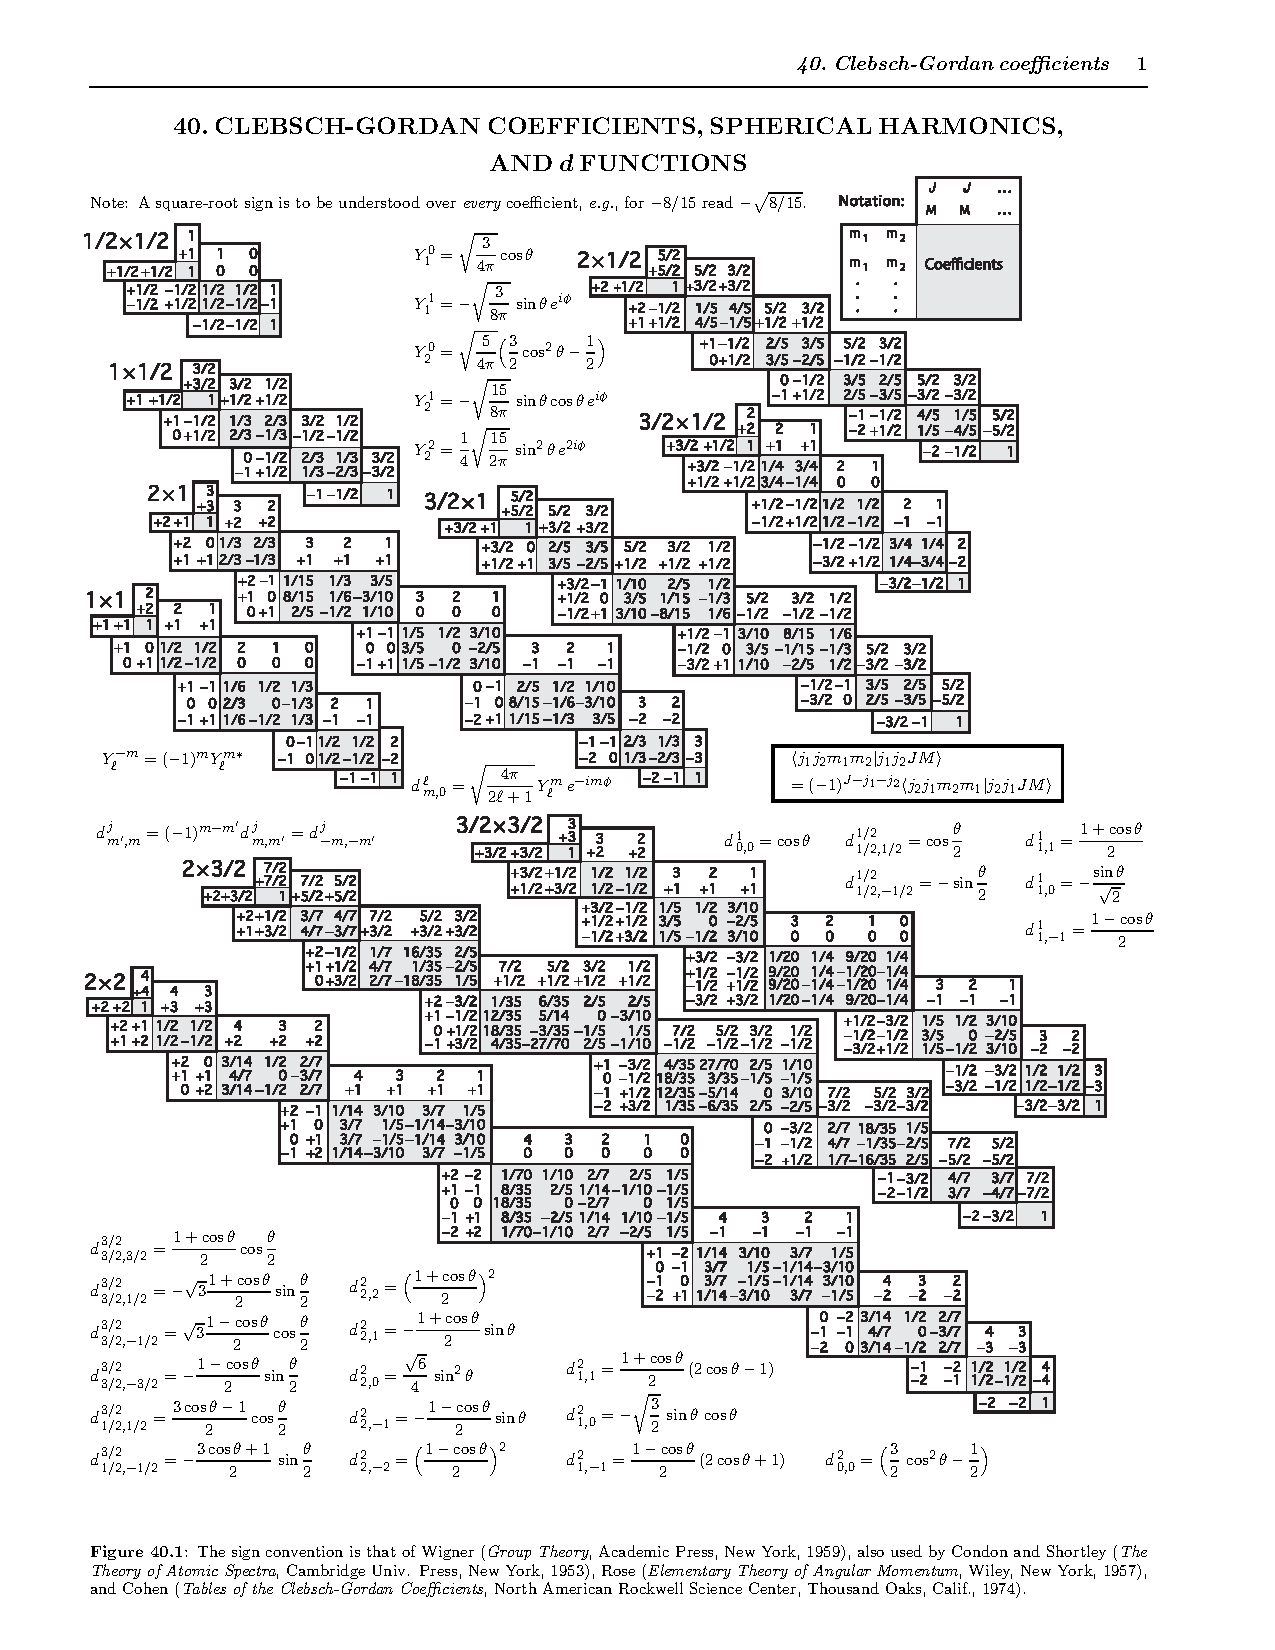
\includegraphics[height=0.9\textheight,keepaspectratio]{CGC}
    \caption{CCG}
    \label{fig:CCG}
\end{figure}
\end{frame}

\subsection{Densit\'a degli stati per N fermioni identici in una scatola}

\begin{frame}{Stati particella in scatola}
Density of available state $\frac{dN}{4\pi p^2dp}$ is given by $dN=4*\frac{4\pi p^2\Omega}{h^3}dp$: we are allowed to place 4 particles in each orbital (spin-isospin).

*Spazio delle Fasi
In un volume dello spazio delle fasi $(2\pi\hbar)^3$ ci stanno al pi\'u $\nu$ particelle dove $\nu$ \'e la degenerazione.

Density of states
Semi-Euristico (Numero di stati fratto volume dello spazio delgi impulsi):

Number of states between $p$ e $p+dp$ is given by $dN=4*\frac{d^3p}{(2\pi\hbar)^3}\Omega=4*\frac{4\pi p^2dp}{(2\pi\hbar)^3}\Omega$.

The infinitesimal thin spherical shell with radius $dp$ has the volume $4\pi p^2dp$.

$g(k)=\frac{dN}{4\pi p^2dp}=\nu\frac{\Omega}{(2\pi)^3}$.

*Stati particella in una scatola
Sia il numero di stati tra $n$ e $n+dn$: $dN=\nu \frac{4\pi n^2dn}{8}$, dove $\nu$ \'e il fattore di degenerazione. La densit\'a di stati fra $k$ e $k+dk$ \'e $g(k)=\frac{dN}{4\pi k^2dk}=\nu \frac{V}{(2\pi)^3}$.

$g(k)=\frac{dN}{4\pi k^2dk}=\nu \frac{V}{(2\pi)^3}$
    
\end{frame}

\begin{wordonframe}{ Density  states for N spin 0 particles in a box}
 
A particle state has volume $h$ in the phase space: we can count particle states as the total phase space volume accessible to that particle divided by the volume of a state. Considero una particella in un volume V (around the scattering center): il numero di stati con momento tra $\vec{p'}$ e $\vec{p'}+d\vec{p'}$ \'e $dn(|\vec{p'}|)=\frac{V*4\pi p^2}{h^3}dp'$ e ho $\rho(E')=\frac{dn(p')}{dE'}=\frac{dn(p')}{v'dp'}=\frac{V*4\pi p^2}{v' h^3}$


\end{wordonframe}

\subsection{Regola d'oro di Fermi}

\begin{frame}{Fermi's golden rule}
 
Probability of transition per unit time: $W_{i\rightarrow f}=\frac{2\pi}{\hbar}|\braket{f|H_{int}|i}|^2\rho(E')$, con $\rho(E')=\frac{dn(E')}{dE'}$.\\
Scattering rate per incident particle and per scattering center: \ev{W_{i\rightarrow f}=\frac{R_b}{N_aN_x}}, with the scattering rate $R_b=\Phi_a\sigma N_x$ ($\phi=n_av_a$): \ev{\sigma=\frac{2\pi}{\hbar v_a}|M_{fi}|^2\rho(E')V}.
Per stati d'onda piana \lbt{\psi_i=\frac{1}{\sqrt{V}}exp(\frac{i\scap{p}{r}}{\hbar})}{\psi_f=\frac{1}{\sqrt{V}}exp(\frac{i\scap{p'}{r}}{\hbar})}
    
\end{frame}


\section{Decadimenti,cinematica (e relativistica)}

\subsection{Decadimenti}

\begin{frame}{Energetica urti/decadimenti}
    \begin{itemize}
\item Equazioni relativistiche per particella $m_1$ incidente su bersaglio fermo $m_2$\\
$\Delta M=\sum_im_{(i)}-(m_1+m_2)$\\
\textbf{Energia CM/LAB}: $E_{cm}=\sqrt{{m_1}^2+{m_2}^2+2\epsilon_{1l}m_2}=\sqrt{({p_1}^{\mu}+{p_2}^{\mu})^2}$\\
\textbf{Energia di soglia nel CM}: ${E_c}^{th}=m_1+m_2+\Delta M$\\
\textbf{Energia di soglia nel Lab}: ${E_{1Lab}}^{th}-m_1=\underbrace{\delta M}_{(-Q)}[1+\frac{m_1}{m_2}+\frac{\Delta M}{2m_2}]$
\item Energia cinetica dei frammenti di un decadimento $\underbrace{A}_M\rightarrow \underbrace{a_1}_{m_1}+\underbrace{a_2}_{m_2}$, nel riferimento di quiete di M.

 Si conservano (c=1) \lbt{\text{Energia: }  M=m_1+m_2+T_1+T_2=e_1+e_2}{\text{Impulso: nel CM }  \vec{0}=\vec{p_1}+\vec{p_2}}
quindi $\underbrace{\vec{p_1}^2}_{e_1^2-m_1^2}=\underbrace{\vec{p_2}^2}_{e_2^2-m_2^2} (M=e_1+e_2) \Rightarrow$\lbt{e_1=\frac{M^2+m_1^2-m_2^2}{2M}}{e_2=\frac{M^2+m_2^2-m_1^2}{2M}}

\end{itemize}

\end{frame}


\section{Collisioni: scattering}

\begin{frame}{Sezione d'urto}
\begin{block}{Numero di urti in $dV$, $dt$.}
\begin{equation*}
    d\nu=\sigma v_{rel}n_1n_2\,dV\,dt
\end{equation*}

The luminosity measures the ability of a particles accelerator to produce the required number of interaction.
 $\# \text{eventi per unit\'a di tempo}=\mathcal{L}\sigma$:\\
$\mathcal{L}=\frac{\text{\# incident particles}}{\text{Area}*\text{Time}}*(\text{\# target particles})=\frac{\text{\# incident particles}}{\text{Time}}\frac{\text{\# target particles}}{\text{Area}}$(Il tutto \'e omogeneo).
\end{block}

\begin{block}{Differential cross section}
$\frac{d\sigma}{d\Omega}=\frac{\text{Events into solid angle $d\Omega$ at $(\theta,\phi)$ per unit time}}{d\Omega*(\text{Incident particles})*(\text{Target nuclei} per cm^2)}$.

Differential Probability of scattering by an angle $\theta$. For each nucleus the probability of scattering by an angle between $\theta$ and $\theta+d\theta$ is equal to the probability of the incident particle having an impact parameter between $b$ and $b+db$: $\frac{dP}{d\theta}d\theta=\frac{dP}{db}db=2\pi bdbN_x=(\text{area per nucleus})*(\text{nuclei per }cm^2)$
\end{block}
Connection between $\frac{d\sigma}{d\Omega}$ and $\frac{dP}{d\theta}$: $N_x\frac{d\sigma}{d\Omega}d\Omega=N_x\frac{d\sigma}{d\Omega}2\pi\sin{\theta}d\theta=\frac{dP}{d\theta}d\theta$.
\end{frame}

\begin{wordonframe}{Angoli Lab-CM (NR)}
    Relazioni sistema Lab ($m_2$ immobile) - sistema CM; $\vec{V}=\frac{m_1\vec{v_1}+m_2\vec{v_2}}{m_1+m_2}$.

Angoli: \lbt{\tan{\theta_1}=\frac{m_2\sin{\chi}}{m_1+m_2\cos{\chi}}}{\theta_2=\frac{\pi-\chi}{2}}.
Velocit\'a: \lbt{\vec{v_1}=\frac{m_2}{m_1+m_2}\vec{v}+\vec{V}}{\vec{v_2}=-\frac{m_1}{m_1+m_2}\vec{v}+\vec{V}}.

Velocit\'a dopo l'urto in Lab in funzione di $\chi$\\
Con $\vec{v}=\vec{v_1}-\vec{v_2}$: 
\lbt{v_1'=\frac{\sqrt{{m_1}^2+{m_2}^2+2m_1m_2\cos{\chi}}}{m_1+m_2}v}{v_2'=\frac{2m_1v}{m_1+m_2}\sin{\frac{\chi}{2}}}.

\end{wordonframe}

\begin{wordonframe}{Sezione d'urto}
$n=$ target atoms per unit volume, $\frac{\rho}{A}N_A$, con $A=$ mass number of target (pure isotope), $\rho x=$ areal density of target $(g/{cm}^2)$, $\rho=$ mass density of target (${g/{cm}^2}$), $nx=$ areal number density $nx=$ areal number density (atoms/$cm^2$) $=\frac{\rho}{A}xN_{Avogadro}$, con $x=$ thickness of target $(cm)$.

 Sia $dR_b$ il numero di particelle scatterate per unit\'a di tempo nell'angolo solido\\ $d\Omega=\sin{\theta} d\theta d\phi$, la sezione d'urto differneziale \'e data da:
 $d\sigma(\Omega)=\frac{dR_b}{I_aN_x}=\frac{1}{I_anx}*\mathcal{F}(\theta,\phi)*\frac{d\Omega}{4\pi}$ con $\int\mathcal{F}(\theta,\phi)\frac{d\Omega}{4\pi}=R_b$.
 
%$\frac{d\sigma}{d\Omega}d\Omega=\frac{\text{\# particelle diffuse per unit\'a di tempo in $d\Omega$}}{\text{\# particelle incidenti per unit\'a di area e di tempo}}$.
%Probabilit\'a che una particella $\alpha$ scatterata incida su un rilevatore di area $A_d$ ad angolo $\theta$: ${A_dN(\theta)}$ ($dN_b(\theta)=I_aN(\theta)A_d, \Delta \sigma=\frac{dN_b}{I_aN_x}$), rimuoviamo la dipendenza dalla geometria del rilevatore dividendo per $\Delta \Omega=\frac{A_d}{r^2}$.

\end{wordonframe}

\subsection{Rutherford scattering}

\begin{frame}{Scattering coulombiano}
Sezione d'urto differenziale per potenziale coulombiano (Formula di Rutherford)
$d\sigma=\pi(\frac{\alpha}{m{v_{\infty}}^2})^2\frac{\cos{\frac{\chi}{2}}}{\sin^3{\frac{\chi}{2}}}=(\frac{\alpha}{2m{v_{\infty}}^2})^2\frac{d\Omega}{\sin^4{\frac{\chi}{2}}}$.

Small deflection angle (region of closest approach: $\Delta x\approx 2b$, $\Delta t\approx\frac{2b}{v}$) The momentum transfer is nearly perpendicular to the incident momentum: $\Delta p_{\perp}\approx \overline{F_{\perp}}\Delta t$.

$\theta\approx\frac{\Delta p_{\perp}}{p}=\frac{2zZ\alpha}{pvb}$ (relativistic) which agrees with non-relativistic calculation $\frac{\theta}{2}\approx\tan{\frac{\theta}{2}}=\frac{zZ\alpha}{2bE_k}=\frac{zZ\alpha}{pvb}$.
Small angle approx: $\frac{d\sigma}{d\Omega}\approx(\frac{2zZ\alpha}{pv})^2\frac{1}{\theta^4}$. 
Frazione di particelle con parametro minore di $b_0$ $f_{b<b_0}=f_{\theta>\theta_0}=\frac{\rho N_A}{M}\pi b_0^2t$.
\end{frame}

\begin{wordonframe}{Scattering Rutherford}
 Scattering angle (small angle), scattering in potenziale coulombiano:
$U(r)=\frac{\alpha}{r}$, Coulomb force on the beam particles with mass $m$ and charge $ze$: $F=\frac{\alpha \hbar c zZ}{r^2}$.

Traiettoria particella $\alpha (ze)$ scatterata da un nucleo $(Ze)$:
$\frac{1}{r}=\frac{1}{b}sin{\phi}+\frac{(ze)(Ze)}{8 \pi \epsilon_0Kb^2}(cos{\phi}-1)$, $K$ energia cinetica della particella $\alpha$ espressa in $eV$ quindi $b=\frac{(ze)(Ze)}{8 \pi \epsilon_0K}cot{\frac{\theta}{2}}$.

\end{wordonframe}

\begin{wordonframe}{Relativistic corrections}

Relazione mass shell: $pc=\sqrt{E^2-(mc^2)^2}$.

Rinculo del nucleo M:
Trascurando la massa $m_e$ dell'elettrone dalla conservazione del 4-momento ho $EMc^2=E'E-\scap{p}{p'}c^2+E'Mc^2$ quindi per l'energia dell'elettrone dopo l'urto $E'=\frac{E}{1+\frac{E}{Mc^2}(1-\cos{\theta})}$.

CEM of a moving charge ($\vec{R}=(X-vt,Y,Z)$) Electric field along direction of motion: $E_{//}=\frac{e}{4\pi\epsilon_0R^2}(1-\frac{v^2}{c^2})$.

Electric field perpendicular to the direction of motion: $E_{\perp}=\frac{e}{4\pi\epsilon_0R^2}\frac{1}{(1-\frac{v^2}{c^2})^{\frac{1}{2}}}$.

Relativistic correction to EM strenght: In the frame of moving particle the EF in trasverse direction is multiplied by $\gamma$ and in compressed by same factor into a smaller region along the direction of particle motion: $\Delta p_{\perp}\approx\frac{\alpha zZ[\gamma]}{b^2}\frac{2b}{v[\gamma]}$.
\end{wordonframe}


\begin{frame}{Scattering qm}
    \begin{columns}[T]
\begin{column}{0.5\textwidth}
\begin{figure}
    \centering
    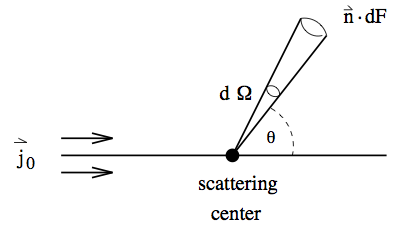
\includegraphics[scale=0.2]{ds}
    \caption{Scattering center: geometry}
    \label{fig:scatgeom}
\end{figure}
\end{column}
\begin{column}{0.5\textwidth}
In termini QM: From the incoming current $\vec{j}_0$ of particles the scattering process create a current $\vec{j}^{sc}$ of scattered particles, $d\sigma=\frac{\vec{j}^{sc}\cdot\hat{n}dF}{|\vec{j}_0|}=\frac{\vec{j}^{sc}\cdot\hat{n}r^2d\Omega}{|\vec{j}_0|}$.
\end{column}
\end{columns}
Soluzione generale per scattering elastico \'e:
 $\braket{\vec{x}|\psi^{\pm}}=\underbrace{\braket{\vec{x}|\phi}}_{\text{onda incidente}}-\underbrace{\frac{2m}{\hbar^2}\int d^3x'\frac{e^{\pm k|\vec{x}-\vec{x'}|}}{4\pi|\vec{x}-\vec{x'}|}\braket{\vec{x'}|V|\psi^{\pm}}}_{\text{Effetto della diffusione}}$.
\end{frame}

\begin{wordonframe}{Scattering ampiezza probabilit\'a}
Lunghezza d'onda di de Broglie: $\lambda=\frac{2\pi \hbar}{p}=\frac{2\pi c\hbar}{pc}=\frac{2\pi (\hbar c)}{\sqrt{E^2-(mc^2)^2}}$.

$\lambdabar=\frac{1}{k}$, $\hbar c\approx 197.3 MeV*fm$.

Optically resolvible object:
per risolvere un oggetto di dimensione caratteristica d con fascio di particelle di lunghezza d'onda $\lambda$ devo avere $\lambda\ll d$.

Corrente di  probabilit\'a: onda piana e funzione d'onda di scattering.

\textbf{Per un'onda piana}: $\vec{J_0}=\frac{\hbar}{m}\Im{[\frac{e^{-\frac{i}{\hbar}\scap{p}{x}}}{(2\pi\hbar)^{\frac{3}{2}}}\nabla(\frac{e^{\frac{i}{\hbar}\scap{p}{x}}}{(2\pi\hbar)^{\frac{3}{2}}})]}=\frac{\frac{p}{m}}{(2\pi\hbar)^3}$\\
\textbf{Per un'onda sferica (scattered wave)}: $\vec{j}^{sc}=|\psi^{sc}|^2v'\hat{n}$.
de Broglie wavelength: $\lambda$ ($\lambdabar=\frac{1}{k}$)\\
$\frac{\lambda}{2\pi}=\frac{\hbar}{p}=\frac{\hbar c}{\sqrt{2mc^2E_{\text{kin}}+E_{\text{kin}}^2}}\approx$\lbt{\frac{\hbar}{\sqrt{2mE_{\text{Kin}}}}\text{ , } E_{\text{Kin}}\ll mc^2}{\frac{\hbar c}{E_{\text{Kin}}}\approx\frac{\hbar c}{E} \text{ , }E_{\text{Kin}}\gg mc^2}.
Cross section:
$\frac{d\sigma}{d\Omega}=(\frac{\overbrace{\alpha}^{(ze)(Ze)}}{4E_{\text{Kin}}})^2\frac{1}{\sin^{\frac{\theta}{2}}}$\\
Per velocit\'a relativistiche:\\
$(\frac{d\sigma}{d\Omega})_{\text{Mott}}=(\frac{d\sigma}{d\Omega})_{\text{Ruth}}(1-\beta^2\sin^2{\frac{\theta}{2}})\abl{v}{c}(\frac{d\sigma}{d\Omega})_{\text{Ruth}}\cos^2{\frac{\theta}{2}}$.\\
Suppression of backscattering ($\theta=\pi$) for target with spin 0 it's a consequence of conservation of helicity.
\end{wordonframe}

\begin{wordonframe}{scattering}
 Urto elastico:
 $H_0\ket{\phi}=E\ket{\phi}. (H_0+V)\ket{\psi}=E\ket{\psi}$, $H=H_0+V, H_0=\frac{\vec{P}^2}{2m}$: in assenza di un centro diffusore, $V=0$, gli autostati sono quelli di $\ket{\vec{P}}$,  per $V\neq0$ gli autostati dell'energia $\neq \ket{\vec{P}}$ tuttavia se il processo d'urto \'e elastico siamo interessati alla soluzione dell'ES per l'hamiltoniana completa con la stessa energia.

Operatore densit\'a di corrente:
Sommo il contribiuto delle funzioni d'onda di tutti i protoni:\\
$\sum_{i=1}^Z|\psiN{Z}|^2\frac{e}{m}\vec{p_i}d^3x_1\ldots d^3x_Z$,\\
 l'integrale \'e su tutte le coordinate eccetto la i-esima e l'elemento della sommatoria relativo \'e il contributo alla corrente dell'i-esimo protone.

\end{wordonframe}

\begin{frame}{Scattering: centro non puntiforme}
    
     \begin{itemize}

\item Born Formula\\
$\frac{d\sigma}{d\Omega}=(\frac{m}{2\pi\hbar^2})^2|\int U(r)e^{i(\vec{k}-\vec{k'})\cdot\vec{x}}d^3x|^2$


\item  Fattore di forma\\
$-Ze^2\int d^3x\int d^3x'\frac{N(r')e^{i\vec{q}\vec{x}}}{|\vec{x}-\vec{x'}|}=Ze^2\frac{4\pi}{q^2}F(\vec{q})$, con \ev{ F(\vec{q})=\int d^3x' e^{i\scap{q}{x'}}N(x')}.

Espansione di $e^{i\scap{q}{x}}$ per piccoli q:
$e^{i\scap{q}{x}}=1+i(\vec{k}-\vec{k'})\cdot\vec{x}-\frac{[(\vec{k}-\vec{k'})\cdot\vec{x}]^2}{2}+\ldots$

Espressione integrale potenziale Coulombiano (Approx. grandi distanze).

\input{coulombdistant}




 \end{itemize}

\end{frame}

\begin{wordonframe}{Scattering di particelle}
 
Sviluppi asintotici:
Per $r=|\vec{x}|\gg r'=|\vec{x'}|$: $e^{\pm ik|\vec{x}-\vec{x'}|}\approx e^{\pm ikr}e^{\mp ik\hat{r}\cdot\vec{x'}}$\\
$\frac{1}{\vec{x}-\vec{x'}}\approx\frac{1}{r}$\\
$|\vec{r}-\vec{r'}|\approx r-\hat{r}\cdot\vec{r'}$\\
In particolare: $\isw{k}{|\vec{r}-\vec{r'}|}\approx\isw{k}{r}e^{-ik\hat{r}\cdot\vec{r'}}$.

Integrale utile per il fattore di forma del potenziale di Yukawa
$\Im{\int_0^{\infty}e^{-\mu r}e^{iqr}dr}=\frac{q}{\mu^2+q^2}$.

FT di $\frac{1}{r}$,
$\int d^3x\frac{e^{i\scap{q}{x}}}{|\vec{x}|}=\frac{4\pi}{q^2}$\\
$\nabla^2\frac{1}{r}=-4\pi\delta^3(\vec{r})$ in trasformata di Fourier diventa $-\vec{q}^2FT(\frac{1}{r})=-4\pi$.

Potenziale come convoluzione: Nel caso il potenziale scatteratore non sia genarato da una carica puntiforme  ma da una distribuzione di carica $\rho(\vec{r})$  il potenziale \'e dato dalla convoluzione $U=\rho\star\frac{1}{r}$.

Impulso trasferito: $q=\frac{2E}{\hbar c}\sin{\theta}{2}$

Esponenziale: $\exp{(\frac{i\scap{q}{r}}{\hbar})}=\sumzi{n}\frac{1}{n!}(\frac{iqr\cos{\theta}}{\hbar})^n$

RK: $E\gg mc^2\Rightarrow E\approx|\vec{p}|c$

\end{wordonframe}

\section{Fisica atomica}


\subsection{Alkali}

\subsection{Helium}

\subsection{Vectorial model}